The projective plane is an idea that grew out of the renaissance study of perspective in art.
For example, when stood between two railway lines, they appear to meet at the horizon. \Cref{projective-parallel} is a rudimentary diagram of the situation.
While this is merely a trick of perspective in euclidean space, in the projective plane, parallel lines \emph{do} meet, at a so called `point at infinity'.
The idea is to add these points at infinity to the euclidean plane so that each line contains exactly one.
On top of this is the one exception, the `line at infinity', which is defined to be the unique line that is simply the collection of all points at infinity.
These ideas, while formative, are hardly rigorous, and we present the proper definition and constructions (there are two) of projective space below.

\begin{figure}[htpb]
	\centering
	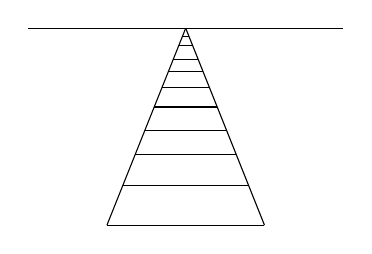
\begin{tikzpicture}[scale=0.5]
		% railway lines
		\draw (-2,0) -- (0,5);
		\draw (2,0) -- (0,5);
		% sleepers. To work out an appropriate x for given y, x=2(1-(y/5))
		\draw (-2,0) -- (2,0);
		\draw (-1.6,1) -- (1.6,1);
		\draw (-1.28,1.8) -- (1.28,1.8);
		\draw (-1.04,2.4) -- (1.04,2.4);
		\draw (-0.8,3) -- (0.8,3);
		\draw (-0.6,3.5) -- (0.6,3.5);
		\draw (-0.44,3.9) -- (0.44,3.9);
		\draw (-0.32,4.2) -- (0.32,4.2);
		\draw (-0.18,4.55) -- (0.18,4.55);
		\draw (-0.08,4.8) -- (0.08,4.8);
		% horizon
		\draw (-4,5) -- (4,5);
	\end{tikzpicture}
	\caption{Parallel lines `meeting' at infinity in euclidean space}
	\label{projective-parallel}
\end{figure}

\begin{definition}
	The projective plane is an extension of regular 2-dimensional euclidean space by adding `points at infinity' such that every pair of lines intersects exactly once. Points in the projective plane are represented as triples of homogenous coordinates [X,Y,Z]. More generally, points in projective $n$-space are represented by $n+1$-tuples, such that not all coordinates are zero.
\end{definition}

The lines given by $2x + 3y + 1 = 0$ and $2x + 3y + 2 = 0$, which are parallel in $\R^2$, intersect in the projective plane at the point [3,-2,0].
This is because, when homogenised with respect to $z$, the curves are given by $2X + 3Y + Z = 0$ and $2X + 3Y + 2Z = 0$, which are clearly satisfied by $[X,Y,Z] = [3,-2,0]$.
The two constructions of projective space give two different interpretations of it, both of which are useful to consider.
% perhaps explain affine space (haha) too?
Projective $n$-space can be thought of as either affine $n$-space with points at infinity added (mentioned already) or as a quotient of affine $(n+1)$-space.

\subsubsection{Construction 1: Quotient of $\an[n+1]$}
Remove the origin (i.e. the point $(0,0,\ldots,0)$) from $\an[n+1]$ and define an equivalence relation on the remaining points as follows:
$$(a_0,a_1,\ldots,a_n) \sim (b_0,b_1,\ldots,b_n) \iff (a_0,a_1,\ldots,a_n) = \lambda(b_0,b_1,\ldots,b_n) = (\lambda b_0,\lambda b_1,\ldots,\lambda b_n)$$
where $\lambda$ is a non-zero scalar.
Then we have 

\subsubsection{Construction 2: Extension of $\an[n]$}
Here is the second construction, blah blah blah...
\lipsum[1-2]
